\chapter{Contexte général du projet}
\label{chap:contexte}

\section{Introduction}
\label{sec:contexte:intro}

\section{Présentation du projet}
\label{sec:contexte:presentation}

\subsection{Cadre du projet}
\label{subsec:contexte:cadre}

\subsection{Objectifs du projet}
\label{subsec:contexte:objectifs}

\subsection{Méthodologie de gestion de projet}
\label{subsec:contexte:methodologie}

% Approche SCRUM adoptée, coordination via Google Meets et WhatsApp, daily meetings

\subsection{Présentation de l'équipe}
\label{subsec:contexte:equipe}

% Tableau des rôles et organigramme fonctionnel

\begin{table}[H]
\centering
\caption{Répartition des rôles au sein de l'équipe}
\label{tab:roles}
\begin{tabularx}{\textwidth}{lclX}
\toprule
\textbf{Rôle} & \textbf{Eff.} & \textbf{Intervenant} & \textbf{Remarque} \\
\midrule
Chef d'équipe / Responsable CI/CD & 1 & \membreUn & Coordination, CI/CD, Dockerisation, validation PR \\
Développeur Fullstack – Infra Cloud & 1 & \membreDeux & Déploiement cloud, environnement de production \\
Développeur Fullstack – Infra Locale & 1 & \membreTrois & Terraform, VMs locales, environnement dev \\
Développeur Fullstack – Sécurité & 1 & \membreQuatre & Keycloak, OWASP ZAP, Trivy, authentification \\
Développeur Fullstack – QA & 1 & \membreCinq & Tests Cypress E2E, tests de charge k6 \\
Développeur Fullstack – Monitoring & 1 & \membreSix & Prometheus, Grafana, observabilité \\
\bottomrule
\end{tabularx}
\end{table}

\begin{figure}[H]
\centering
% 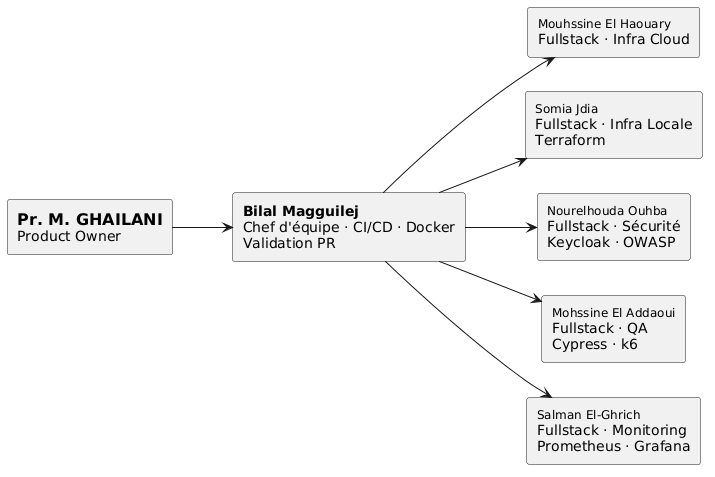
\includegraphics[width=\textwidth]{images/organigramme.png}
\caption{Organigramme fonctionnel de l'équipe}
\label{fig:organigramme}
\end{figure}

\subsection{Planification du projet}
\label{subsec:contexte:planification}

% Diagramme de Gantt prévisionnel et réel

\begin{figure}[H]
\centering
% \includegraphics[width=\textwidth]{images/gantt-previsionnel.png}
\caption{Diagramme de Gantt prévisionnel}
\label{fig:gantt-previsionnel}
\end{figure}

\begin{figure}[H]
\centering
% 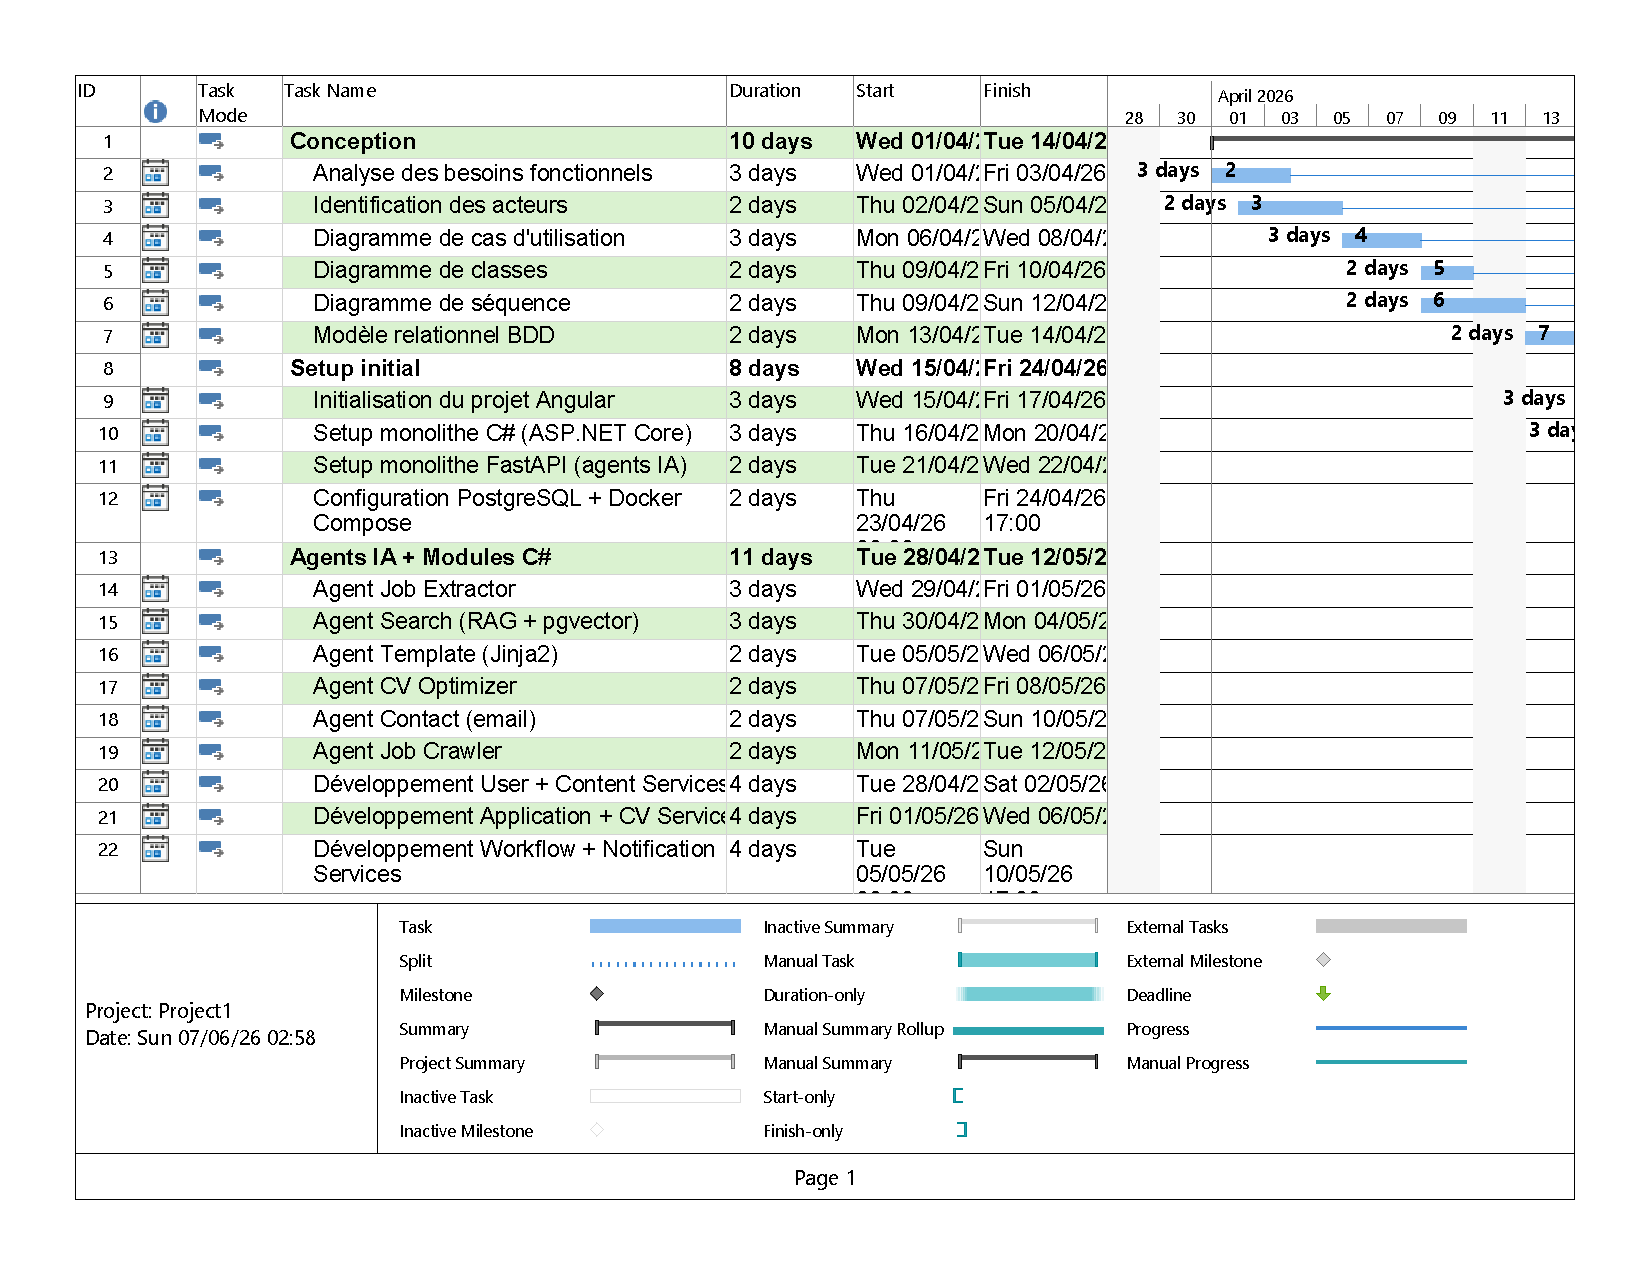
\includegraphics[width=\textwidth]{images/gantt-reel.png}
\caption{Diagramme de Gantt réel}
\label{fig:gantt-reel}
\end{figure}

\section{Conclusion}
\label{sec:contexte:conclusion}
